\section{Introduction}
In this paper the field, \(\mathbb{F}\), will be used to denote the real field, \(\mathbb{R}\), and the complex field, \(\mathbb{C}\).
The triangle inequality is a fundamental concept which provides crucial relationships between distances for various structures within mathematics. 
The triangle inequality states that for any triangle, the sum of the lengths of any two sides must be greater than or equal to the length of the remaining side. 
Formally, one can state:
\[
d(A, C) \leq d(A, B) + d(B, C).
\]
\begin{example}
    Consider the following triangle:
    \begin{center}
       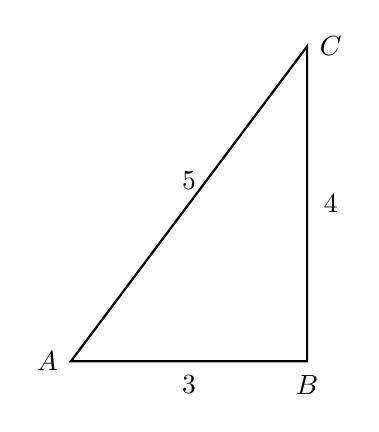
\begin{tikzpicture}
        % Draw the triangle
        \draw[thick] (0, 0) -- (3, 0) -- (3, 4) -- cycle;
        % Label the sides
        \node at (1.5, -0.3) {3};
        \node at (3.3, 2) {4};
        \node at (1.5, 2.3) {5};
        % Label the angles
        \node at (-0.3, 0) {$A$};
        \node at (3, -0.3) {$B$};
        \node at (3.3, 4) {$C$};
    \end{tikzpicture} 
\end{center}
 Clearly, 
$
5 \leq 3 + 4 = 7,
$
indicating the triangle inequality holds true for this example.
\end{example}

When this relationship is generalized to the real number line or complex plane, the magnitude from any number to zero results in the absolute value or modulus, respectively.
Therefore, the triangle inequality can be rewritten as follows for any $a,b \in \mathbb{F}$:
%%Maybe state the other conditions that triangle inequality have to satisfy here,
\[|a + b| \leq |a| + |b|
\]
This inequality, which always holds true in this particular field, extends naturally to matrices. The absolute value (or modulus) of a matrix  $A$ , 
denoted as  $|A| = \sqrt{A^*A}$ , is defined for any $ A \in \mathbb{M}_n(\mathbb{F})$. Given this definition, one might reasonably conjecture that
\[
|A + B| \leq |A| + |B|
\]
would similarly hold for matrices  \(A, B \in \mathbb{M}_n(\mathbb{F}).\) However, this is not always the case, and the triangle inequality can indeed fail for matrices, as noted by \cite{BK} and others.
Understanding the rate and conditions under which the triangle inequality is valid is crucial, as it have significant implications for the analysis of boundedness and convergence properties in matrix theory. 
\par This paper seeks to explore and quantify the likelihood of these failures, thereby providing deeper insights into the structural behavior of the effects of matrix absolute value on the triangle
inequality. 
Thorough investigation into sets
\begin{itemize}
    \item \(\mathbb{M}_n\left(\mathbb{Z} \cap \left\{ (-k, \ldots, k) \;\middle|\; k \in \mathbb{Z} \right\}\right)\),
    \item \(\mathbb{M}_n\left(\mathbb{Z}[i] \cap \left\{ x + i y \;\middle|\; x, y \in (-k, \ldots, k), \; k \in \mathbb{Z} \right\}\right)\),
    \item \(\mathbb{M}_n\left(\mathbb{R} \cap \left\{ [-k, k] \;\middle|\; k \in \mathbb{R} \right\}\right)\), and
    \item \(\mathbb{M}_n\left(\mathbb{C} \cap \left\{ x + i y \;\middle|\; x, y \in [-k, k], \; k \in \mathbb{R} \right\}\right)\)
\end{itemize}
 was conducted numerically using an error tolerance of \(10^{-7} \) to determine their frequency of failure.
Restricting the entry ranges allows for more control and is insightful on the behavior on the triangle inequality on the absolute value; therefore, any further discussion on the triangle
inequality will be focused on \(\mathbb{M}_n\) unless otherwise stated.